\documentclass[preprint,12pt]{article}

\usepackage{algorithmic}
\usepackage{algorithm}
\usepackage{enumerate}
\usepackage{enumitem}
\usepackage{graphics}
\usepackage{graphicx}
\usepackage{geometry}
\usepackage{amsmath}
\usepackage{wrapfig}
\usepackage{subfig}
\usepackage{framed}
\usepackage{color}
\usepackage{soul}
\usepackage{bm}

\usepackage{multirow}
\usepackage[T1]{fontenc}
\usepackage[latin9]{inputenc}
%\usepackage{units}
\usepackage{esint}

\geometry{legalpaper,  margin=1in}

\newcommand{\CM}[2][green]{ {\sethlcolor{#1} \hl{#2}} }
\newcommand{\KB}[2][cyan]{ {\sethlcolor{#1} \hl{#2}} }

%\makeatother

%\usepackage{babel}fs

\begin{document}
\title{Extracting the components of Specific Partisan Asymmetry for Wisconsin Assembly 2010 census cycle districts}
\author{Kevin Baas and Colin McAuliffe}
\maketitle

\section{Method}

To compare how much of the observed partisan asymmetry in 2010-cycle Wisconsin State Assembly districsts was the result of changes in district designs versus changes in voter sentiment, we varied the first while holding the second constant.

For this analysis we used official districting plans for the 2000 and 2010 census cycles, and actual vote counts from the 2006, 2008, 2010, 2012, 2014, and 2016 assembly elections, at precinct-level resolution, imputing uncontested elections with partisan swing matched presidential election results when available, and partisan swing matched federal congress election results when not.
By "partisan swing matched" we mean that the Republican vote counts in all districts are multiplied by a constant factor so that the total vote count matches that for the assembly elections, for the subset of districts in which both elections were contested, and the same is done for the Democratic vote counts.
Then election data for 2006, 2008, and 2010 was cross-aggregated at census block resolution to the 2010-cycle districts, and election data for 2012, 2014, and 2016 was cross-aggregated at census block resolution to the 2000-cycle districts. 
 
Since the same exact elections are used in both the 2000 districts analysis and 2010 districts analysis, \emph{all} differences in the results are the consequnece of the redistricting scheme used, and conversely, changes in voter sentiment have exactly \emph{zero} contribution to the difference.

Furthermore, if the 2000 census cycle districts show a partisan asymmetry much lower than the 2010 cycle, then we know that natural "political geography" -- the tendency of Democratic voters to be clustered in cities -- was \emph{not} a significant factor in the partisan asymmetry inherent in 2010 cycle Wisconsin Assembly districts, since any contributions from political geography would be present in \emph{both} districting schemes.
However, if they are not substantially different, this would not demonstrate that political geography was a significant contribution, because they both could be artificially gerrymandered on top of any unintentional gerrymandering due to political geography.

\section{Measurement}
To measure partisan bias, we measured the asymmetry in the seats-votes curve at the actual vote count that occured in the election.  
In other words, we take the number of seats that Republicans won, and subtract from that the number of seats that Democrats would have won if the popular vote percentage was reversed (1-x), and divide by 2.  
This represent the number of seats Republicans won in excess of what they would have won if the seats-votes curve was symmetric.  
If the number is negative, that represents an asymmetry in favor of Democrats.
We call this "specific partisan asymmetry".

\subsection{Advantages of this metric}
 
Before applying this metric to concretes example, we'd like to highlight some of the advantages of it.

\begin{itemize}

\item Doesn't assume proportionality in results - The seats-votes curve for single-winner elections naturally take on a cumulative Beta-binomial distribution, as opposed to a diagonal line representing seats proportional to votes.  This metric doesn't assume a diagonal curve representing proportionality.  It tests a looser (less strict) criteria: asymmetry, which still retains the essential feature of measuring disenfranchisement based on political belief.  SCOTUS has ruled that seats proportional to votes can not be a legal standard (Thornburg v. Gingles 1986).   But they remain open to a legal standard based on the idea of partisan symmetry.
 
\item Distinguishes between artificial partisan bias and the natural multiplying effect of single-winner elections -  Single-winner aka "Majoritarian" elections naturally over-favor the majority party, giving them a larger fraction of the seats than they get of the popular vote.  
While some measures might mistakenly identify this as gerrymandering, specific asymmetry explicitly takes this into account by calculating and then subtracting this natural multiplying effect.
In other words, it does not mistake disproportionality due to the sigmoidal shape of marjoritian election seats-votes curves with gerrymandering.

\item Works for states with partisanship far from 50/50 - By sampling the asymmetry at the actual vote counts rather than e.g. 50/50, this metric maintains full relevance even for the most extremely partisan states.

\item Represents deviation from what is practically achievable - It is trivial for a computer algorithm to design districts that make the seats-votes curve perfectly symmetric, while satisfying all constitutional requirements.  
Thus, to convert this absolute score to one relative to what can be accomplished by a redesign that meets all traditional redistricting principles, one simply subtracts zero.  
This "new" relative score gives you the number of voters whose votes were effectively stolen by the map drawers with the current map, and whose right to representation can be returned by a remedy map that can be trivially designed by a computer employing a multi-objective heuristic optimization algorithm.

\item The only possible improvements are shift, scale, and shape - Since it is well ordered and monotonic with respect to actual partisan advantage, any "better" measure can only be better in the sense of having a more appropriate "center" point, a more appropriate scale, or a more appropriate "shape" (change of slope as you go up and down the scale).  The scale varies from -1 to 1, or alternatively from negative the number of seats available to the positive of that.  The "center",  zero, is a non-arbitrary and very reasonable choice, representing a perfectly symmetric situation.   The "shape" is the number (or percentage) of congressional seats affected.

\item It gives a result in an empirically meaningful unit: number of seats, which can be directly converted into number of ballots/voters affected by multiplying by the number of ballots cast and dividing by the number of districts.

 
 
\end{itemize}


\section{Past elections}


\section{Future elections}


Before applying this model to a concrete examples, we'd like to highlight some of the advantages of it.


\subsection{Probability model}

\subsection{Advantages of this model}
 
\begin{itemize}

\item Takes into account non-uniform swings - By looking at not only the average partisanship of each district, but how much the partisanship of each individual district changes from election to election, this metric is able to take into account the changes in voter sentiment that are not uniform throughout the state; that are perhaps concentrated in only certain districts.

\item It takes into account all possibilities, weighted by likelihood - Every possible seats-votes curve and every possible popular vote ratio is taken into consideration, weighted by the combined likelihood of the two.

\item Shows durability - By computing an entire likelihood function for specific partisan asymmetry, rather than a single point estimate, this metric enables quick and accurate assessment of how durable a gerrymander is; how much more harm it will cause in the future, including what the likelihood is that it will not cause harm.

\end{itemize}


\section{2010 districts results}
\subsection{Future election result likelihoods (District partisanship likelihoods)}
 
Shown in figure \ref{fig:Betas} is a graph of district partisanship, including dispersion.  To generate this graph, a Beta distribution for each district was calculated using the method of moments.  Additionally a Beta distribution for the total popular vote was calculated using the method of moments.  Then the probability density function was plotted out for each one of them.  (The black curve in the middle is the total popular vote.) Results that lead to a Democrat winning the seat are colored in blue, and results that lead to a Republican winning the seat are colored in red.
Note, in addition to the the average of the past 6 elections, the graph also shows the statistical dispersion, from which the durability of this effect for future elections can be assessed.

\begin{figure}[htb!]
    \begin{center}
        \includegraphics[scale=0.25]{../Figures/WI2010/Betas_cropped.png}
        \caption{Beta distributions for Wisconsin 2010-cycle Assembly districts}\label{fig:Betas}
    \end{center}
\end{figure}
 
Note that Democratic-leaning districts are both far to the right, showing high partisanship (and thus low voter impact), and low dispersion -- meaning the voters are unlikely to change their minds; they are "safe" Democratic voters.  Conversely, the Republican-leaning districts are closer to the middle, but still safely to the left, and all centered around about the same place.   These are characteristic signs of Betag.  Let me rephrase that: this is the very definition of "packing and cracking".  The Democratic voters were packed - hence far to the left.  By concentrating Democratic voters in few districts, this reduces the number of seats that Democratic voters can win.  The remaining population was "cracked" to get the Republican-leaning districts all to about the same level of moderately (but safely) Republican-leaning partisanship, thus increasing the number of seats that Republican voters can win.  The net effect is to maximize the impact of Republican votes, and minimize the impact of Democratic votes.
 
Shown in figure \ref{fig:SVAssembly} are twelve seats-votes curves drawn from these distributions (solid curve), along with their 2-axis reflection (dashed curve), and a popular vote percentage drawn from the statewide Beta distribution (vertical dotted gray line).  A large and consistent asymmetry in favor of Republicans is immediately evident.

\begin{figure}[htb!]
    \begin{center}
        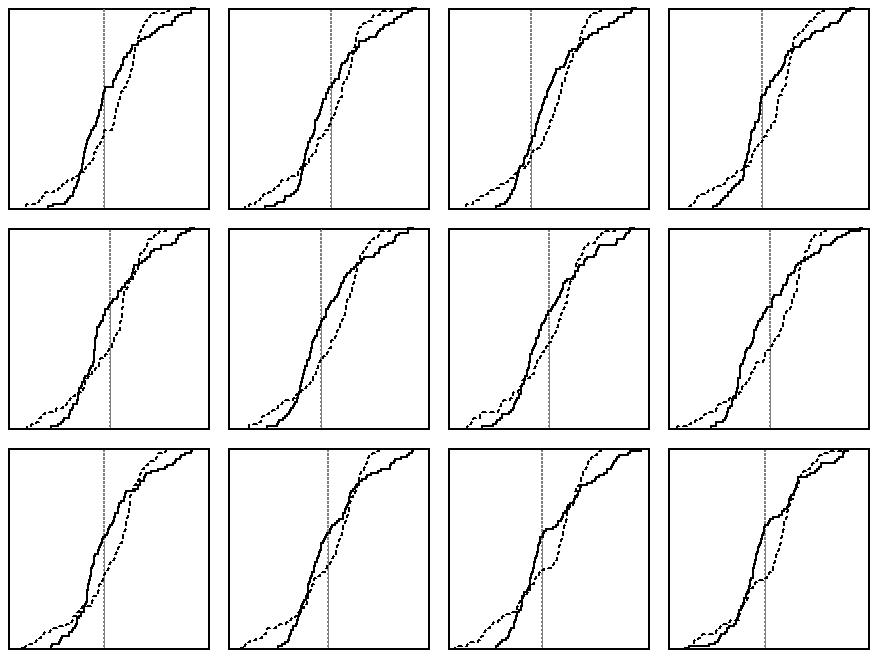
\includegraphics[scale=0.5]{../Figures/WI2010/sv_curves_assembly.png}
        \caption{Some election outcome seats-votes curves generated from the probability model for Wisconsin 2010 Assembly districts}\label{fig:SVAssembly}
    \end{center}
\end{figure}

\subsection{Numerical integrations of likelihood functions}

\subsubsection{Specific partisan asymmetry likelihoods}
 
To get the likelihood function for partisan asymmetry, we use Monte-Carlo numerical integration, subtracting the seat counts Democrats would get with that share of the vote from the number Republicans would get under the same share of the vote, and then dividing by 2. The results are shown in figure \ref{fig:LikelihoodsAsymmetry}, as a fraction of total available seats.
 
\begin{figure}[htb!]
    \begin{center}
        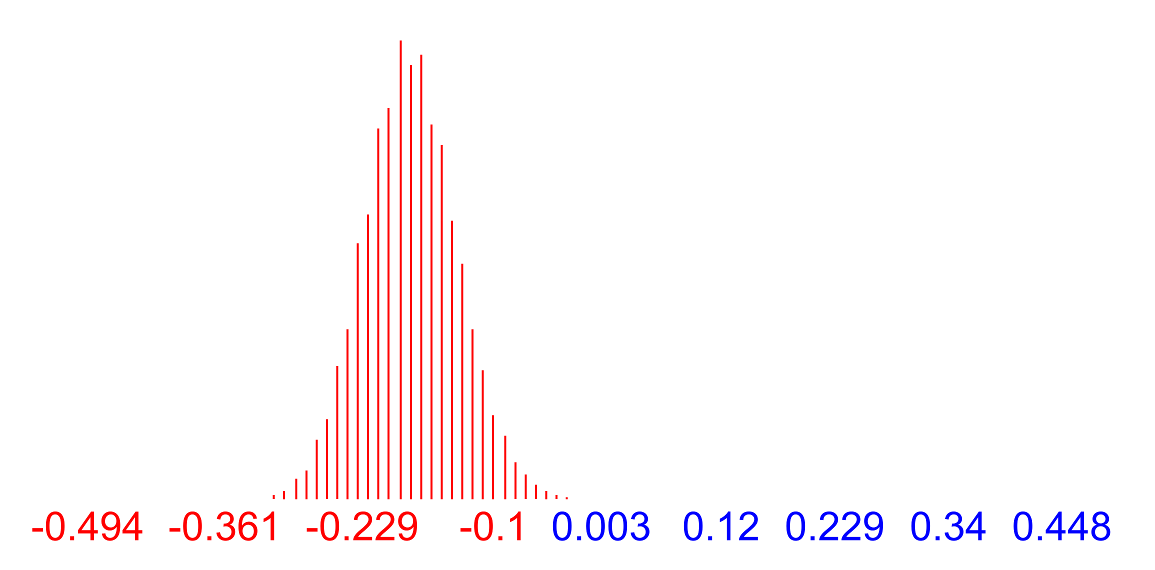
\includegraphics[scale=0.5]{../Figures/WI2010/asymmetry_alt.png}
        \caption{Specific asymmetry likelihoods generated from the probability model for Wisconsin 2010 Assembly districts}\label{fig:LikelihoodsAsymmetry}
    \end{center}
\end{figure}
 
Note the mode of the distribution - the most likely result - is a partisan asymmetry of 20\% of the available seats.  For instance, the most likely result might be that Republicans get 6/10ths of the legislative seats, whereas if the popular vote count were reversed, Democrats would get only 4/10th of the legislative seats.  Remedying this would give Democrats 10\% more seats.  This means that roughly 10\% of the entire Democratic-voting population of the state of Wisconsin were effectively disenfranchised, in violation of the one person, one vote principle.  Conversely, 10\% of the Republican-voting population effectively got an extra vote.  That's approximately 306,000 felonies.
 
Note, out of 100,000 sample points, none of them resulted in specific partisan asymmetry favoring Democrats.  Since an assembly district election occurs every 2 years, this shows that, without significant changes in geo-spatial demographics, the asymmetric pro-Republican partisan advantage inherent in this redistricting will persist for the next 200,000 years.

\subsubsection{District partisanship histogram}
 
Another way we can see this is by looking at the histogram of district partisanship.
 
Similarly to how we modeled vote percentages with Beta distributions, we used Gamma distributions to model voter turnout.  We then combined these two to model actual vote counts in each district.  This allowed us to compute likelihood functions for specific vote counts in every district.  We then used Monte Carlo integration to construct the likelihood function for district partisanship, over all districts.
 
The resulting curve shown in figure \ref{fig:LikelihoodsDistrictPartisanship} leaves no room for interpretation.  The high red peak close to the center but still safely to the side shows that Republican districts are heavily cracked.  Conversely, the mass of blue far to the side and comparative lack of a strong peak close to the center shows that Democratic districts are heavily packed.
 
\begin{figure}[htb!]
    \begin{center}
        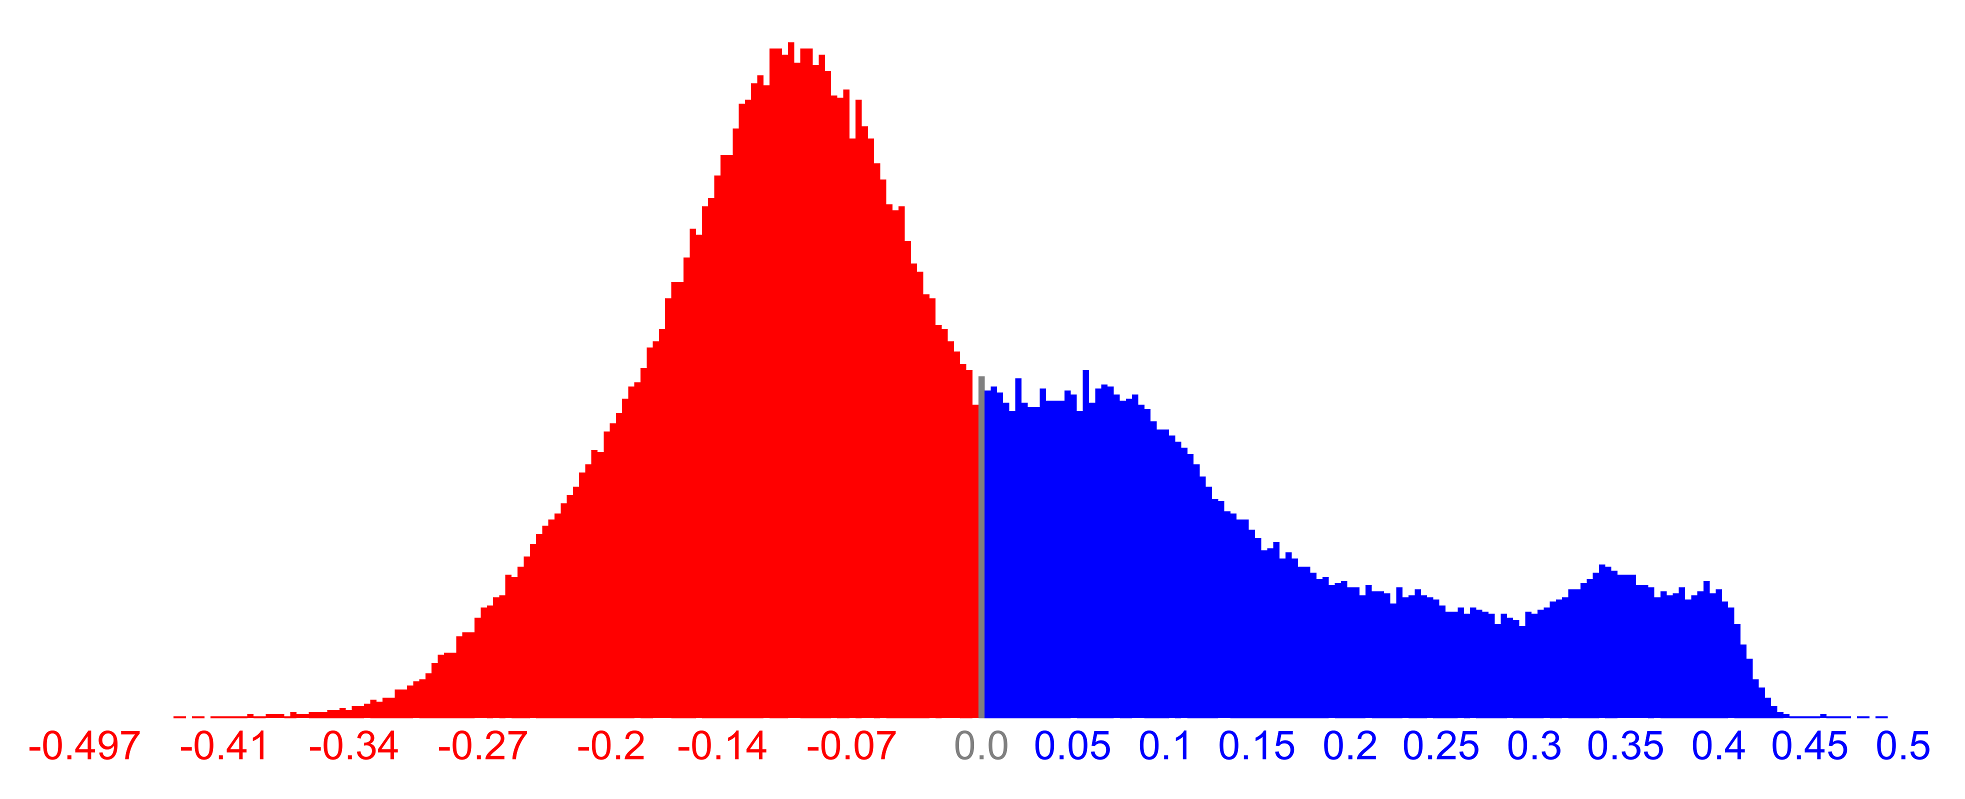
\includegraphics[scale=0.25]{../Figures/WI2010/district_partisanship_cropped.png}
        \caption{District partisanship likelihoods generated from the probability model for Wisconsin 2010 Assembly districts}\label{fig:LikelihoodsDistrictPartisanship}
    \end{center}
\end{figure}

\subsubsection{Statewide seat count likelihoods}
 
The seat count likelihoods produced by this packing and cracking can be shown by integrating the statewide and district partisanship likelihood functions.  As these distributions, like most Bayesian models, don't lend themselves to analytic integration, numerical integration must be used. Using the Monte-Carlo numerical integration method, with 100,000 samples, we constructed the probability mass function for the Republican seat count results from an election, given the current districts and voter demographics.  The results are shown in figure \ref{fig:LikelihoodsSeatCounts}.
 
Particularly striking about this result is that, while the popular vote likelihoods in the above graph centers around 50/50, favoring Democratic representatives more than 40\% of the time, the seat count likelihoods never put Democratic representatives in the majority.  Indeed, out of 100,000 samples, it never even gives them 42 out of 99 of the seats.  On average Republican representatives maintain a 60-39 seat advantage.   This shows a sizable and durable partisan advantage for Republicans, despite the actual voters showing no clear preference, and indeed, preferring Democrats almost half the time.

\begin{figure}[htb!]
    \begin{center}
        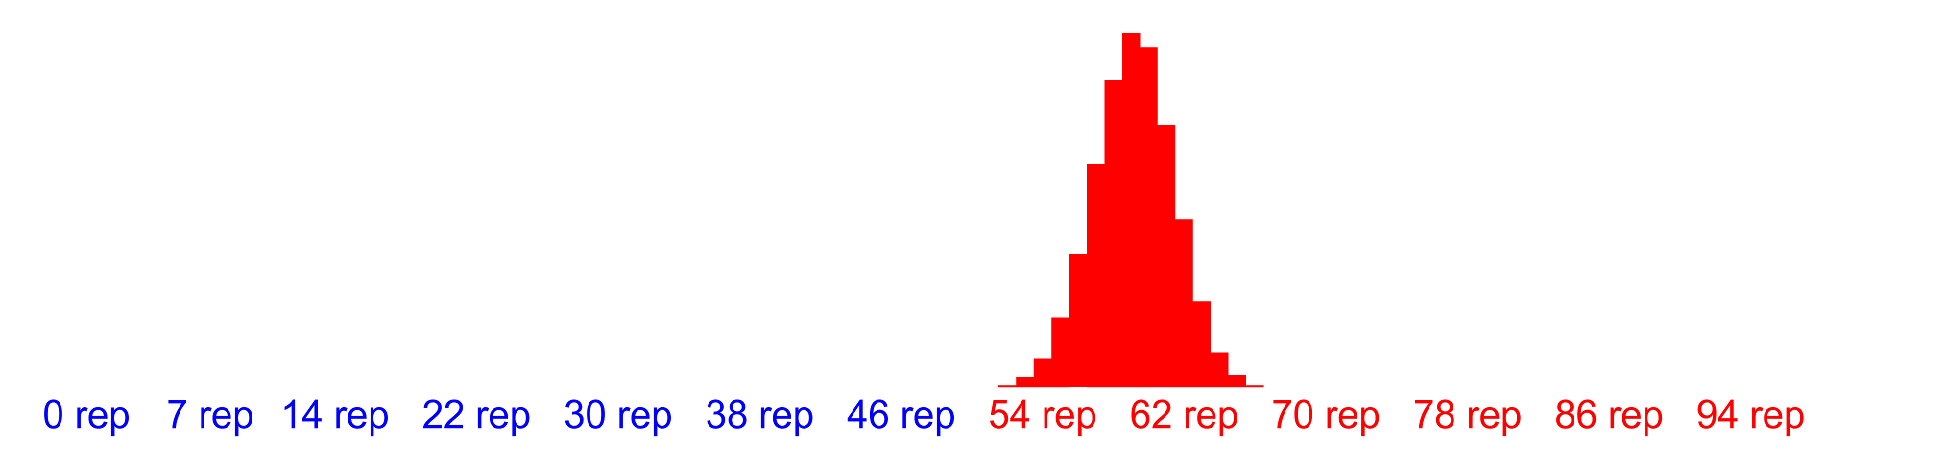
\includegraphics[scale=0.3]{../Figures/WI2010/seats_cropped.png}
        \caption{Seat count likelihoods generated from the probability model for Wisconsin 2010 Assembly districts}\label{fig:LikelihoodsSeatCounts}
    \end{center}
\end{figure}
 
\section{Comparison}

\section{Conclusions}
From these comparisons, it is painfully obvious that the specific partisan asymmetry present in the 2010 cycle districts is \emph{not} present in the 2000 cycle districts, even when using vote count data from the exact same elections.  Therefore:
\begin{itemize}
\item Since the same exact voter sentiments were used in both analyses, this difference in partisian asymmetry simply cannot be a consequence of changes in voter sentiment.  Since the only thing that we changed was the districting scheme, all observed differences in partisan asymemtry are purely the result of changing the districting scheme.
\item Natural political geography was \emph{not} a significant factor in the partisan asymmetry inherent in Wisconsin Assembly districts in the 2010 cycle.  Were this a significant factor, the exact same effects would be present in the 2000 districts, but they are not.  This finding is consistent with Professor Jowei Chen's findings in his paper "The Impact of Political Geography on Wisconsin Redistricting: An Analysis of Wisconsin's Act 43 Assembly Districting Plan".
\item Simply reverting back to the 2000 census cycle districts would remedy most of the present injustice, as measured in seats affected or ballots affected.
\end{itemize}



%\bibliographystyle{plainnat}
\bibliographystyle{unsrt}
\bibliography{gerrymandering}
\clearpage



\end{document}
